\begin{question}
\noindent A biologist is tracking a bacterium specimen on a microscope slide. The slide is modelled as a coordinate grid, where each unit represents 1 micrometre.

\noindent The specimen's outline is triangle $S$ with vertices $A(-4,1)$, $B(-4,4)$ and $C(-2,1)$, as shown below.

\begin{center}
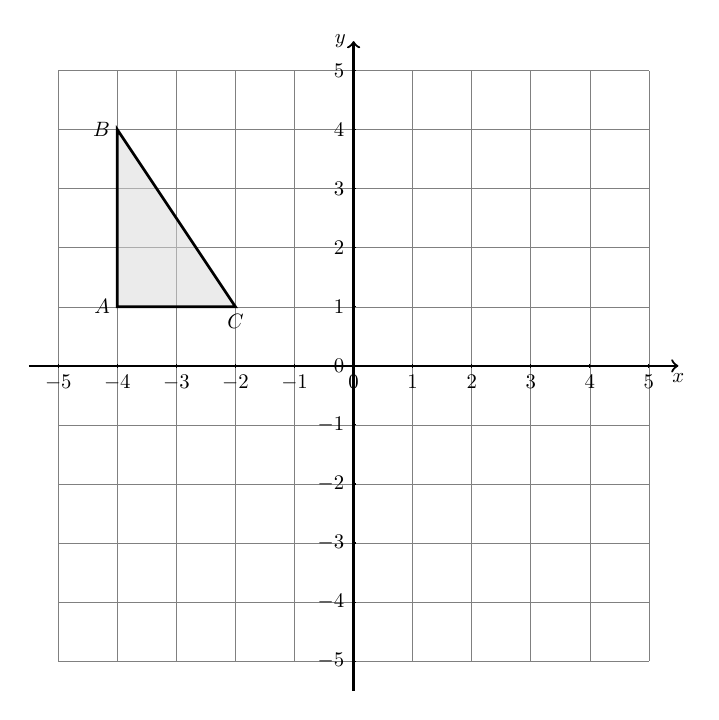
\begin{tikzpicture}[scale=0.75, transform shape]
    \definecolor{borderColour}{HTML}{000000}
    \definecolor{fillColour}{HTML}{D8D8D8}

    \def\axisLimit{5}

    \draw[step=1cm,gray,very thin] (-\axisLimit,-\axisLimit) grid (\axisLimit,\axisLimit);

    \draw[thick,->] (-\axisLimit-0.5,0) -- (\axisLimit+0.5,0) node[anchor=north] {$x$};
    \draw[thick,->] (0,-\axisLimit-0.5) -- (0,\axisLimit+0.5) node[anchor=east] {$y$};

    \foreach \x in {-\axisLimit,...,\axisLimit}
        \draw (\x cm,1pt) -- (\x cm,-1pt) node[anchor=north] {$\x$};
    \foreach \y in {-\axisLimit,...,\axisLimit}
        \draw (1pt,\y cm) -- (-1pt,\y cm) node[anchor=east] {$\y$};

    \coordinate (A) at (-4,1);
    \coordinate (B) at (-4,4);
    \coordinate (C) at (-2,1);

    \filldraw[fill=fillColour, draw=borderColour, line width=1pt, fill opacity=0.5] (A) -- (B) -- (C) -- cycle;

    \node[left] at (A) {$A$};
    \node[left] at (B) {$B$};
    \node[below] at (C) {$C$};

\end{tikzpicture}
\end{center}

\noindent The biologist first records the specimen after it drifts across the slide with translation vector $\begin{pmatrix} 3 \\ -2 \end{pmatrix}$, forming triangle $S'$.

\noindent She then notices the microscope's image is mirrored, so triangle $S'$ must be reflected in the line $x = 1$ to give the correct orientation, triangle $S''$.

\noindent Work out the coordinates of the vertices of triangle $S''$.
\vspace{5cm}
\begin{flushright}
\answerplain{3}
\end{flushright}
\end{question}
